\documentclass[grado3]{LEMA-Tikz-IM}

\usepackage{graphicx}  % Needed to include graphics
% \usepackage{pifont} % For the scissors symbol

\begin{document}
\begin{tikzpicture}
% \pgfplotsset{compat=1.18}

% page canvas letter size
\path (0,0) rectangle (8.5in,11in);

% draw cut line
% \usetikzlibrary{decorations.text}
% \node at (0.5in, 11in/2) {\scalebox{2}{\ding{36}}};
% \node at (8.5in-0.5in, 11in/2) {\scalebox{2}{\ding{36}}};
% \draw[dashed, line width=1pt] (0,11in/2) -- (8.5in, 11in/2);

\def\myMargin{1in}

\coordinate (botLeft) at (\myMargin,\myMargin);
\coordinate (botRight) at (8.5in-\myMargin,\myMargin);
\coordinate (topRight) at (8.5in-\myMargin,11in-\myMargin);
\coordinate (topLeft) at (\myMargin,11in-\myMargin);

% clip outside the margin 
\clip (botLeft) rectangle (topRight);


% find center of the page
\coordinate (center) at ($ (botLeft)!0.5!(topRight) $);

% add tables to top and bottom
\node (tarjetas) at ([yshift=-2ex]center) {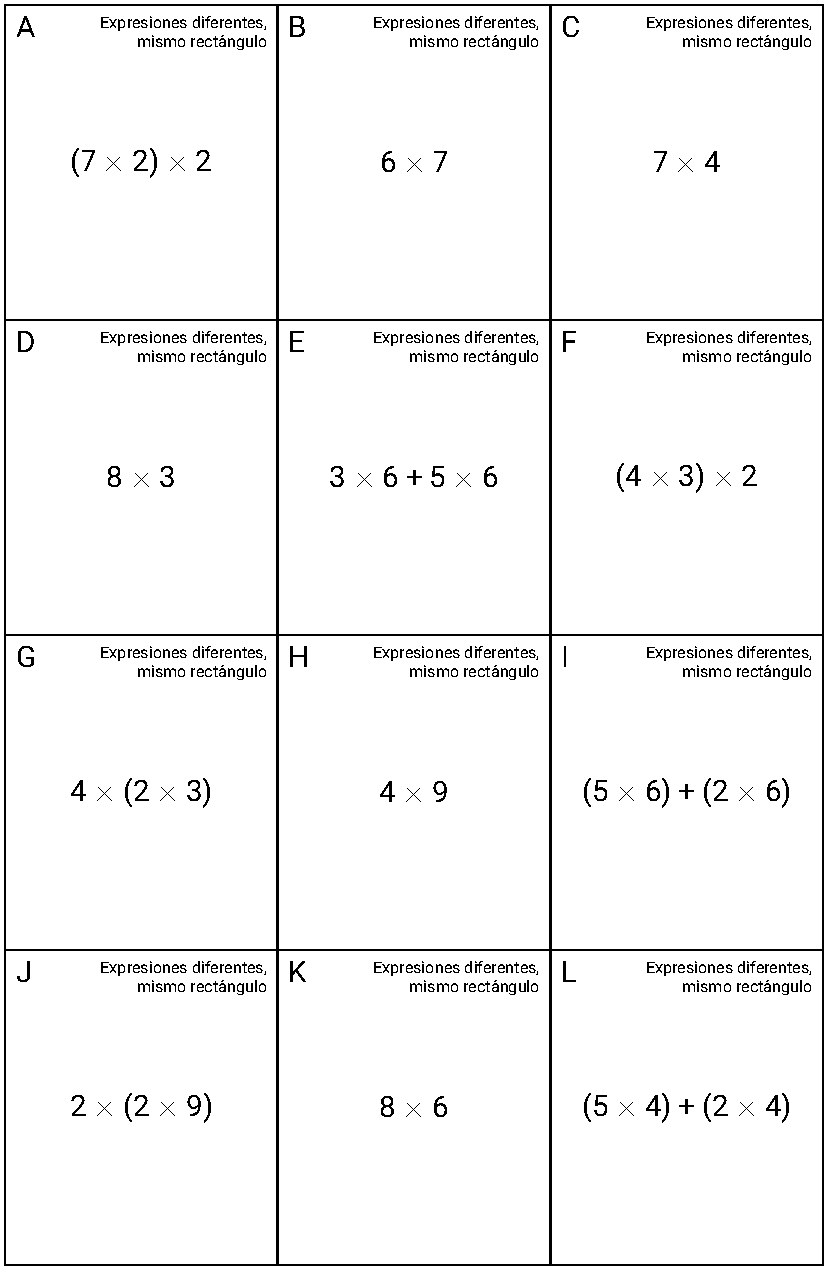
\includegraphics{clasificacionTarjetas-expresionesDiferentesMismoRect-tarjetas.pdf}};


% Add BLM heading
\node[below right, font=\bf\LARGE] at ([]topLeft) {Expresiones diferentes, mismo rectángulo};



\end{tikzpicture}
\end{document}